%
% ACMD 2026 abstract -- Terramechanics-Aware Shared Control for Off-Road
% Teleoperation on Deformable Terrain.
% Submission file name (per template): ShaZhouSerban_abstract.pdf
%
\documentclass{acmd2026_abstract}

\usepackage{float}
\usepackage{xurl}
\setlength{\emergencystretch}{3em}

\graphicspath{{images/}{paper_figures/}}

\begin{document}

%------------------------------------------------------------
% title
\begin{center}
  \fontsize{14}{10}{\bf
    Terrain-Aware, Latency-Robust Control \\
    for Off-Road Autonomy and Teleoperation
  }
\end{center}
\vspace{-6pt}

%------------------------------------------------------------
% authors  (speaker = Kyle Sha is underlined per template)
\begin{center}
\normalsize{
  \bf{
    \underline{Kyle Sha},
    Zhenhao Zhou,
    Radu Serban,
    Dan Negrut}
}
\end{center}
\vspace{-6pt}

%------------------------------------------------------------
% affiliations  (single affiliation -- reference marks omitted)
\begin{center}
  \begin{tabular}{c}
    Department of Mechanical Engineering             \\
    University of Wisconsin--Madison                 \\
    1513 University Ave., Madison, WI 53706, USA     \\
    \{kasha2, zzhou292, serban, negrut\}@wisc.edu    \\
  \end{tabular}
\end{center}
\vspace{-8pt}

%------------------------------------------------------------
% abstract
\section*{Abstract}
We present a real-time, latency-aware human-in-the-loop framework
for safe shared and autonomous control of vehicles on deformable
Soil Contact Model (SCM)~\cite{Krenn09} terrain.  A differentiable
neural surrogate of the SCM tire forces is embedded inside an
acados NMPC for terrain-aware trajectory tracking, while a
learned online estimator regresses the dominant soil parameters
from onboard IMU and wheel-speed signals so that both the NMPC
and a latency-aware DOB-CBF-QP safety filter track the terrain and
compensate time-varying teleoperator delay in real time.  We simulate an HMMWV on
SCM terrain using Chrono::Vehicle (Project Chrono~\cite{Tasora16});
Chrono::Sensor supplies driver POV and a Logitech G29 steering/pedals.
Simulator, NMPC, terrain estimator, and CBF-QP exchange data over
low-latency ZMQ; ML-based 5G models~\cite{Choi23}
inject delay only on the camera and human-control paths, not between
simulator and controller.

\vspace{2pt}
\noindent\textbf{Contributions.}  Off-road
teleoperation must contend with deformable-soil effects~\cite{Bekker69}
that rigid-terrain tire models cannot capture without per-deployment
recalibration~\cite{Dallas21}, while time-varying network
latency~\cite{Choi23} requires latency-aware shared-control
arbitration~\cite{Zhang25}.  Building on Project Chrono~\cite{Tasora16} and
the human-in-the-loop framework Chrono::HIL~\cite{Zhou23}, we contribute: (i)~a differentiable
neural SCM tire surrogate that augments the static MLP
of~\cite{Dallas21} with rate-augmented and ResNet variants and
exposes a peak longitudinal traction budget $F_x^{\mathrm{trac}}$
to the NMPC as $|M a_x|\!\le\!F_x^{\mathrm{trac}}$ ($M$ vehicle
mass, $a_x$ commanded longitudinal acceleration), paired with an
asymmetric throttle DOB on the actuation map that closes the
residual soft-soil speed gap left by open-loop $\dot u\!=\!a_x$
with $u$ longitudinal speed;
(ii)~a learned online terrain estimator that
replaces the UKF of~\cite{Dallas21} and jointly regresses
Bekker~$n$ and Mohr--Coulomb~$\phi$ from onboard IMU and
wheel-speed signals, conditioning both the surrogate and the
traction-aware NMPC constraints online; (iii)~a two-layer obstacle-avoidance
stack that pairs in-horizon NMPC softplus barriers with a
downstream latency-aware DOB-CBF-QP safety
filter~\cite{Zhang25} whose friction cone is tightened by the same
$\phi$ estimate; and (iv)~an open-source parallelized
data-collection and benchmarking suite that scales training and
closed-loop evaluation across terrains and reference trajectories.

\section*{Technical content}
\vspace{-4pt}

\noindent\textbf{Human-in-the-loop stack.}  Chrono::Vehicle~\cite{Serban19}
runs an HMMWV on an SCM patch within Chrono::HIL~\cite{Zhou23}.
The human views Chrono::Sensor driver POV and steers a Logitech G29
via \texttt{pygame} with SDL2 haptics.  IMU measurements ride on the
ZMQ vehicle-state stream to NMPC and the terrain estimator.  A second
process runs NMPC and CBF-QP on low-latency ZMQ to the sim;~\cite{Choi23}
delays hit the simulated camera stream and operator commands
(Fig.~\ref{fig:sysArch}); one workstation closes the loop in real
time.

\begin{figure}[H]
  \vspace{-6pt}
  \begin{center}
    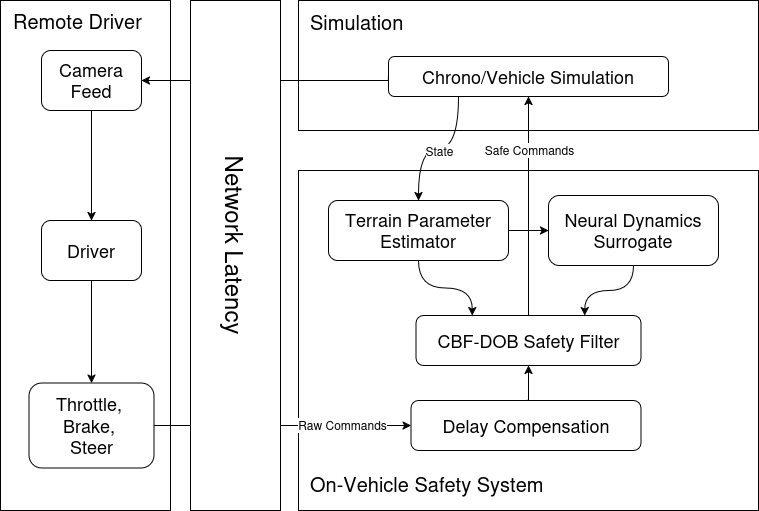
\includegraphics[width=0.44\textwidth]{Sys Arch v4.drawio.png}\hfill
    
\includegraphics[width=0.55\textwidth]{bench_tire_models.png}
    \caption{\small \textbf{Left:} shared-control architecture:
      SCM surrogate and learned terrain estimator inform the NMPC and
      the DOB-CBF-QP filter that screens delayed operator inputs.
      \textbf{Right:} NMPC tracking at $5$\,m/s (LC and sinusoid,
      $2$\,m amp, $30$\,m wavelength); RMS crosstrack error (m),
      mean$\pm$std, $5$ runs/cell.}
    \label{fig:sysArch}
  \end{center}
  \vspace{-10pt}
\end{figure}

\noindent\textbf{Differentiable SCM surrogate.}  A small neural network
maps $(\kappa,\alpha,F_z,u)$, steering rate, and soil parameters
$\boldsymbol{\theta}_{\mathrm{soil}}\!=\!(K_\phi,K_c,n,c,\phi,k)$
(Bekker--Wong--style rig inputs~\cite{Shibly05}) to longitudinal and
lateral tire forces.  Where~\cite{Dallas21} employ a static MLP, we add
rate-augmented and ResNet variants (Fig.~\ref{fig:sysArch}, right);
all train on parallelised Project Chrono SCM tire-rig sweeps and export as
CasADi expressions so acados auto-differentiates through the tire
forces every solve step.  The longitudinal traction cap
$F_x^{\mathrm{trac}}$ queries the surrogate at reference slip
$\kappa_{\mathrm{ref}}$ with $\alpha\!=\!0$, using axle loads
$F_z$, speed $u$, and
$\boldsymbol{\theta}_{\mathrm{soil}}$ from terrain presets or
the online estimator.  Cornering forces $F_y$ use the same
$\boldsymbol{\theta}_{\mathrm{soil}}$ but the live operating point
$(\kappa,\alpha,F_z,u)$ at each NMPC stage.

\noindent\textbf{Online terrain estimation.}  Where
Dallas~et al.~\cite{Dallas21} drive an Unscented Kalman filter
through their NN tire model, we train a window MLP that regresses
Bekker~$n$ and Mohr--Coulomb~$\phi$ from a few seconds of onboard
IMU and wheel-speed history, using dimensionless coupling channels
that make the descriptor approximately speed-invariant.  Trained on a mixed open- and
closed-loop corpus, the estimator converges within seconds on
canonical clay, dirt and sand (Fig.~\ref{fig:terrainEstimator}),
generalises to randomly sampled unseen soils, and re-conditions the
surrogate online so that closed-loop tracking improves by an order of
magnitude over Pacejka and TMeasy (Fig.~\ref{fig:sysArch}, right).
Rich-excitation LHS data support joint $(n,\phi)$ regression (held-out
RMSE $\approx\!0.07$ in $n$, $\approx\!3.3^{\circ}$ in $\phi$);
ensemble disagreement on $\phi$ gates the safety filter's friction
cone.

\noindent\textbf{NMPC barriers and delay-aware safety filter.}
Obstacle handling uses two complementary layers.  (i)~The NMPC
adds a smooth softplus barrier (stage and terminal) over live-$\phi$
traction limits, proactively re-planning inside its horizon.
(ii)~A downstream DOB-CBF-QP safety filter~\cite{Zhang25} screens
autonomous and operator commands via a heading-aligned ellipsoidal
barrier elongated ahead of the vehicle: a filter-side first-order
velocity DOB captures unmodelled SCM drag, the NN surrogate sets the
traction-limited top speed, and the barrier plus forward-prediction
collision check are inflated by an EMA teleoperation round-trip
delay drawn from the same 5G model~\cite{Choi23}.

\begin{figure}[H]
  \vspace{-6pt}
  \begin{center}
    
\includegraphics[width=0.50\textwidth]{closed_loop_estimator_learned.png}
    \caption{\small Convergence of $\hat n$ on canonical
      clay/dirt/sand under closed-loop NMPC at $5$\,m/s.}
    \label{fig:terrainEstimator}
  \end{center}
  \vspace{-10pt}
\end{figure}

\noindent\textbf{Open-source data and benchmarks.}  Parallelized SCM sweeps for training
and a benchmark suite across terrains and reference trajectories;
per-process ZMQ enables running the Fig.~\ref{fig:sysArch} $6\times 6$ grid
($180$ NMPC trials) in under $30$\,min on one workstation.

\vspace{-6pt}
%------------------------------------------------------------
% bibliography  (alphabetical, ACMD style)
\enlargethispage{28pt}
{\scriptsize
\raggedright
\sloppy
\begin{thebibliography}{aber}
\setlength{\itemsep}{-5pt}
\setlength{\parsep}{0pt}
\setlength{\topsep}{-6pt}
\setlength{\labelsep}{0.5em}

\bibitem[1]{Bekker69}
  Bekker, M.G.: Introduction to Terrain-Vehicle Systems.
  \newblock University of Michigan Press, Ann Arbor, 1969.

\bibitem[2]{Choi23}
  Choi, Y.-H.~et al.: ML-based 5G traffic generation for practical simulations using open datasets.
  \newblock IEEE Commun.\ Mag., Vol.~61, pp.~130--136, 2023.
  \newblock doi: \url{https://doi.org/10.1109/MCOM.001.2200679}.

\bibitem[3]{Dallas21}
  Dallas, J.~et al.: Terrain adaptive trajectory planning and tracking on deformable terrains.
  \newblock IEEE Trans.\ Veh.\ Technol., Vol.~70, No.~11, pp.~11255--11268, 2021.
  \newblock doi: \url{https://doi.org/10.1109/TVT.2021.3114088}.

\bibitem[4]{Krenn09}
  Krenn, R.; Hirzinger, G.:
  SCM -- a soil contact model for multi-body system simulations.
  \newblock ISTVS, Bremen, 2009.

\bibitem[5]{Serban19}
  Serban, R., Taylor, M., Negrut, D., Tasora, A.: Chrono::Vehicle: template-based ground vehicle modelling and simulation.
  \newblock Int.\ J.\ Veh.\ Perf., Vol.~5, No.~1, pp.~18--39, 2019.

\bibitem[6]{Shibly05}
  Shibly, H., Iagnemma, K., Dubowsky, S.: An equivalent soil mechanics formulation for rigid wheels in deformable terrain.
  \newblock J.\ Terramech., Vol.~42, No.~1, pp.~1--13, 2005.
  \newblock doi: \url{https://doi.org/10.1016/j.jterra.2004.05.002}.

\bibitem[7]{Tasora16}
  Tasora, A.~et al.: Chrono: an open source multi-physics dynamics engine.
  \newblock HPCSE, pp.~19--49, Springer, 2016.
  \newblock doi: \url{https://doi.org/10.1007/978-3-319-40361-8_2}.

\bibitem[8]{Zhang25}
  Zhang, H.~et al.: Shared control of teleoperated vehicles with delay-compensated safety filtering.
  \newblock IEEE CCTA, pp.~192--199, 2025.

\bibitem[9]{Zhou23}
  Zhou, Z.~et al.: A Chrono-based framework for large-scale traffic simulation with human-in-the-loop.
  \newblock 2023.
  \newblock doi: \url{https://doi.org/10.13140/RG.2.2.23133.59361}.

\end{thebibliography}
\par
}

\end{document}
